\subsection{Distance to Lines}

Next up is the distance between points and lines. The shortest distance between a point and a line in $\bbr^3$ should certainly be along the path perpendicular to the line, but unfortunately we don't have a great way to generate the direction vector between the line and the point. So we need to do something a little different. 

\begin{claim}{Point to Line}
Consider a line $L$ and a point $P$ such that $P$ does not lie on $L$ (if $P$ lies on $L$ then the distance is zero). Let $L$ have a direction vector of $\vcd$. Then we can draw a line segment from $P$ to $L$ such that that line segment is perpendicular to $L$.
\vspace{1em}
\begin{center}
\begin{tikzpicture}
%	\draw[->, color=red,line width=0.5mm](0,0)--(5,3);
	\draw[<->,line width=0.5mm](-4,0)--(8,0);
%	\draw[->, color=purple,line width=0.7mm](0,0)--(5,0);
	\draw[dashed, line width=0.5mm](5,3)--(5,0);
	\draw[](5,0.3)--(4.7,0.3)--(4.7,0);
	\node at (5,3) {$\bullet$};
	\node at (5.5,3.5) {$P$};
%	\node[color=red] at (2.5,2) {$\vcw$};
	\node at (-0.5,0.5) {$L$};
%	\node[color=purple] at (3,0.5) {$\proj{\vcw}{\vcv}$};
\end{tikzpicture}
\end{center}
\vspace{1em}
Call the point where this perpendicular line segment intersects the line $R$, and then pick an arbitrary point $Q$ on $L$. These three points form the right triangle $\triangle PQR$. Call $\angle PQR=\theta$.
\vspace{1em}
\begin{center}
\begin{tikzpicture}
%	\draw[->, color=red,line width=0.5mm](0,0)--(5,3);
	\draw[<->,line width=0.5mm](-4,0)--(8,0);
%	\draw[->, color=purple,line width=0.7mm](0,0)--(5,0);
	\draw[dashed, line width=0.5mm](5,3)--(5,0);
	\draw[](5,0.3)--(4.7,0.3)--(4.7,0);
	\node at (5,3) {$\bullet$};
	\node at (5.5,3.5) {$P$};
%	\node[color=red] at (2.5,2) {$\vcw$};
	\node at (-1.5,0.5) {$L$};
	\node at (0,0) {$\bullet$};
	\node at (0,-0.5) {$Q$};
	\node at (5,0) {$\bullet$};
	\node at (5,-0.5) {$R$};
	\draw [line width=0.5mm](0,0)--(5,3);
	\draw (0.5,0) arc (0:30:0.5);
	\node at (0.8,0.25) {$\theta$};
%	\node[color=purple] at (3,0.5) {$\proj{\vcw}{\vcv}$};
\end{tikzpicture}
\end{center}
\vspace{1em}
By SOH-CAH-TOA, we know that $$\frac{||\overline{PR}||}{||\overline{PQ}||}=\sin\theta.$$
Also, $||\overline{PR}||$ is the distance we are trying to find, while we can find $||\overline{PQ}||$ by taking the vector difference of the vectors that represent $P$ and $Q$. So we get that the distance between our point and our line can be found using $$d=||\vcp-\vcq||\sin\theta .$$
Finally, we invoke the cross product formula from Theorem 1.4.5, noting that $\theta$ is the angle between $\vcp-\vcq$ and $\vcd$, so:
\begin{align*}
||(\vcp-\vcq)\times\vcd||=&||\vcp-\vcq||\cdot ||\vcd||\sin\theta\\
\frac{||(\vcp-\vcq)\times\vcd||}{||\vcp-\vcq||\cdot ||\vcd||}=&\sin\theta.
\end{align*}
Then by substitution:
\begin{align*}
d=&||\vcp-\vcq||\sin\theta\\
=&||\vcp-\vcq||\frac{||(\vcp-\vcq)\times\vcd||}{||\vcp-\vcq||\cdot ||\vcd||}\\
d=&\frac{||(\vcp-\vcq)\times\vcd||}{ ||\vcd||}
\end{align*}
\end{claim}

\begin{claim}{Point to Line Algorithm}
\begin{enumerate}
\item Find the direction vector for your line, call it $\vcd$.
\vspace{1em}
\item Call the point $P$, represented by vector $\vcp$. Then pick an arbitrary point $Q$ on your line, represented by vector $\vcq$.
\vspace{1em}
\item Find the vector between $P$ and $Q$ as the vector difference $\vcp-\vcq$.
\vspace{1em}
\item Find your distance $d$ as $$d=\frac{||(\vcp-\vcq)\times\vcd||}{ ||\vcd||}. $$
\end{enumerate}
\end{claim}

\begin{exercise}{Point to Line}
Find the distance between the following points and lines.
\vspace{1em}
\begin{enumerate}
\item \href{https://www.geogebra.org/3d/skreh6sd}{Let $P$ be the point $(2,1,-3)$ and $L(t)=\bmat{1\\-1\\4}t+\bmat{0\\1\\0}.$ (Geogebra Link)}
\vspace{1em}
\item \href{https://www.geogebra.org/3d/sfhumpus}{Let $P$ be the point $(1,1,1)$ and $L$ be the line with symmetric form $\dfrac{x}{2}=y-1=2z+1.$ (Geogebra Link)}
\end{enumerate}
\end{exercise}

Our very last case to deal with is the distance between two lines in $\bbr^3$. This is the most complicated case, because there are actually multiple subcases. As usual, if the lines intersect, then the distance is zero. But we have to treat the case where the two lines are parallel a little differently than the two cases where the lines are \textit{skew} to each other.

\begin{exercise}{Parallel, Skew, or Intersect?}
For the following lines, decide if they are parallel, skew, or intersecting lines.
\vspace{1em}
\begin{enumerate}
\item Let $\vec{L}_1(t)=\bmat{1\\2\\3}t+\bmat{0\\0\\-1}$ and $L_2(t)=\bmat{2\\-3\\-1}t+\bmat{1\\2\\2}$. Hint: Set $\vec{L}_1(t)=\vec{L}_2(s)$. Then solve the system of equations presented by the first two coordinates, then check to see if those values of $s$ and $t$ satisfy the third coordinate!
\vspace{1em}
\item Let $L_1(t)=\bmat{2\\3\\-1}t+\bmat{3\\3\\1}$ and $L_2(t)=\bmat{4\\6\\-2}t+\bmat{1\\0\\0}$.
\vspace{1em}
\item Let $\vec{L}_1$ be the line with symmetric form $x=2y-1=3z+1 $ and $\vec{L}_2$ be the line with symmetric form $x-2=\dfrac{y}{2}=2z.$
\end{enumerate}
\end{exercise}

In the parallel case, both lines are contained in some plane. So then you can just pick a point $P$ along one of the two lines, and then proceed with the point to line plan.
\begin{center}
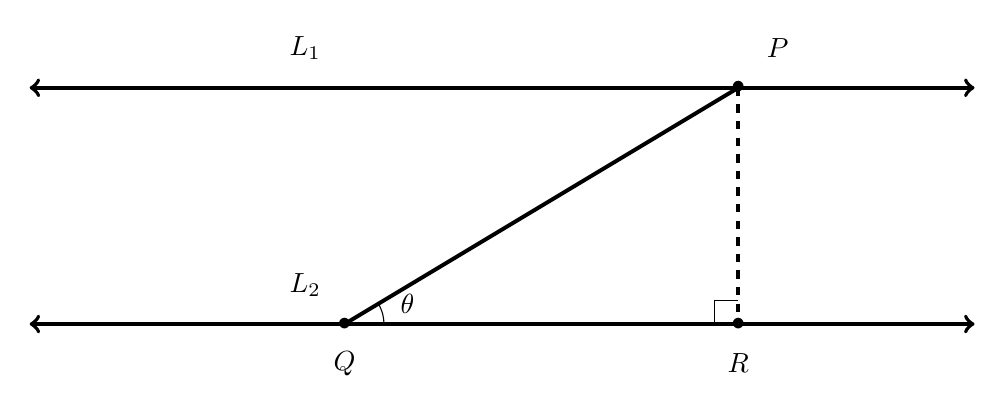
\begin{tikzpicture}
%	\draw[->, color=red,line width=0.5mm](0,0)--(5,3);
	\draw[<->,line width=0.5mm](-4,0)--(8,0);
	\draw[<->,line width=0.5mm](-4,3)--(8,3);
%	\draw[->, color=purple,line width=0.7mm](0,0)--(5,0);
	\draw[dashed, line width=0.5mm](5,3)--(5,0);
	\draw[](5,0.3)--(4.7,0.3)--(4.7,0);
	\node at (5,3) {$\bullet$};
	\node at (5.5,3.5) {$P$};
%	\node[color=red] at (2.5,2) {$\vcw$};
	\node at (-0.5,0.5) {$L_2$};
	\node at (-0.5,3.5) {$L_1$};
	\node at (0,0) {$\bullet$};
	\node at (0,-0.5) {$Q$};
	\node at (5,0) {$\bullet$};
	\node at (5,-0.5) {$R$};
	\draw [line width=0.5mm](0,0)--(5,3);
	\draw (0.5,0) arc (0:30:0.5);
	\node at (0.8,0.25) {$\theta$};
%	\node[color=purple] at (3,0.5) {$\proj{\vcw}{\vcv}$};
\end{tikzpicture}
\end{center}

\begin{claim}{Line to Line Algorithm (parallel)}
\begin{enumerate}
\item Pick an arbitrary point $P$ on one of your lines and an arbitrary point $Q$ on the other line. Call $\vcd$ the direction vector of one of your lines.
\vspace{1em}
\item Proceed with the point to line algorithm.
\end{enumerate}
\end{claim}

\begin{exercise}{}
Why does it not matter which of the two lines we take $\vcd$ from?
\end{exercise}

\begin{exercise}{Line to Line (parallel)}

Find the distance between the following lines.
\vspace{1em}
\begin{enumerate}
\item \href{https://www.geogebra.org/3d/h4zqcru5}{Let $L_1(t)=\bmat{2\\3\\-1}t+\bmat{3\\3\\1}$ and $L_2(t)=\bmat{4\\6\\-2}t+\bmat{1\\0\\0}$. (Geogebra Link)}
\vspace{1em}
\item \href{https://www.geogebra.org/3d/zzu9vwnf}{Let $L_1$ be the line with symmetric form $x=2y-1=\dfrac{z}{2} $ and $L_2$ be the line with symmetric form $x+1=2y=\dfrac{z+4}{2}.$ (Geogebra Link)}
\end{enumerate}
\end{exercise}

Lastly, we consider the case where we have two lines that are \textit{skew} to each other. That is, they are not parallel but do not intersect.

\begin{exercise}{Skew Lines and Parallel Planes}
Consider two lines, $L_1$, which has parametric form $$L_1(t)=\bmat{t\\t\\0}$$ and $L_2$ which has parametric form $$L_2(t)=\bmat{t\\-t\\2}. $$
\begin{enumerate}
\item Find $\vcd_1$, the direction vector for $L_1$ and $\vcd_2$, the direction vector for $L_2$.
\vspace{1em}
\item How can we tell that $L_1$, $L_2$ are not parallel?
\vspace{1em}
\item Pull up the graph of these two lines on \href{https://www.geogebra.org/3d/dwvfymu7}{Geogebra 3D}.
\vspace{1em}
\item Graph the two parallel planes, $z=0$ and $z=2$ in that same Geogebra 3d window. Verify that your two lines are contained in these two planes and the two planes are parallel.
\vspace{1em}
\item Use $\vcd_1$, $\vcd_2$ and the point $(0,0,0)$ to generate the parametric form of a plane. Then convert that parametric plane to standard form and verify that it is, in fact, the plane $z=0$.
\vspace{1em}
\item Use $\vcd_1$, $\vcd_2$ and the point $(0,0,2)$ to generate the parametric form of a plane. Then convert that parametric plane to standard form and verify that it is, in fact, the plane $z=2$.
\end{enumerate}
\end{exercise}

The idea contained in the previous exercise generalizes. In fact, given two skew lines, we can always generate two parallel planes, one containing each line, which reduces us to the plane to plane case. We can algorithmically kinda mash some steps together to get us straight to good old point to plane.

\begin{claim}{Line to Line Algorithm (skew)}
\begin{enumerate}
\item Call your two lines $L_1$, $L_2$. Find the two direction vectors, $\vcd_1$, $\vcd_2$.
\vspace{1em}
\item Find a point $Q$ on $L_1$. Then generate the plane that contains $L_1$ that is parallel to $L_2$ by using the two direction vectors $\vcd_1$, $\vcd_2$ and containing $Q$.
\vspace{1em}
\item Pick an arbitrary point $P$ on $L_2$, then proceed with point to plane algorithm.
\end{enumerate}
\end{claim}

\begin{exercise}{Line to Line (skew)}
Find the distance between the following lines.
\vspace{1em}
\begin{enumerate}
\item \href{https://www.geogebra.org/3d/js6pygd7}{Let $\vec{L}_1(t)=\bmat{1\\1\\-1}t+\bmat{2\\4\\1}$ and $\vec{L}_2(t)=\bmat{-2\\1\\3}t+\bmat{1\\1\\3}$. (Geogebra Link)}
\vspace{1em}
\item \href{https://www.geogebra.org/3d/y349fgsf}{Let $\vec{L}_1$ be the line with symmetric form $x=2y-1=3z+1 $ and $L_2$ be the line with symmetric form  $x-2=\dfrac{y}{2}=2z.$(Geogebra Link)}
\end{enumerate}
\end{exercise}